\documentclass[11pt,a4paper]{article}
% no creation date or random file ID in the PDF, so a rebuild gives the same bytes
\ifdefined\pdfinfoomitdate\pdfinfoomitdate=1\pdftrailerid{}\fi
\usepackage[margin=2.1cm]{geometry}
\usepackage[T1]{fontenc}
\usepackage{lmodern}
\usepackage{microtype}
\usepackage{graphicx}
\usepackage{booktabs}
\usepackage{tabularx}
\usepackage{longtable}
\usepackage{array}
\usepackage{enumitem}
\usepackage{xcolor}
\usepackage[font=small,labelfont=bf]{caption}
\usepackage{float}
\usepackage[hidelinks]{hyperref}
\setlist{itemsep=2pt,topsep=3pt}
\setlength{\parskip}{4pt}\setlength{\parindent}{0pt}
% generated by make_numbers.py from data/*.csv -- do not edit
\expandafter\def\csname v@abs.cap60_bH0.random\endcsname{0}
\expandafter\def\csname v@abs.cap60_bH0.switch\endcsname{0}
\expandafter\def\csname v@abs.slow_bH0.random\endcsname{49.5}
\expandafter\def\csname v@abs.slow_bH0.switch\endcsname{49.5}
\expandafter\def\csname v@ad.0.3.f\endcsname{13.0}
\expandafter\def\csname v@ad.0.3.fr\endcsname{$-$2.7}
\expandafter\def\csname v@ad.0.3.gap\endcsname{1.5}
\expandafter\def\csname v@ad.0.3.k\endcsname{6}
\expandafter\def\csname v@ad.0.3.o\endcsname{11.5}
\expandafter\def\csname v@ad.0.3.phrase\endcsname{2.7 questions slower}
\expandafter\def\csname v@ad.0.3.r\endcsname{15.7}
\expandafter\def\csname v@ad.0.3.rr\endcsname{1}
\expandafter\def\csname v@ad.0.6.f\endcsname{11.4}
\expandafter\def\csname v@ad.0.6.fr\endcsname{$-$0.5}
\expandafter\def\csname v@ad.0.6.gap\endcsname{3.2}
\expandafter\def\csname v@ad.0.6.k\endcsname{4}
\expandafter\def\csname v@ad.0.6.o\endcsname{8.2}
\expandafter\def\csname v@ad.0.6.phrase\endcsname{0.5 questions slower}
\expandafter\def\csname v@ad.0.6.r\endcsname{11.9}
\expandafter\def\csname v@ad.0.6.rr\endcsname{1}
\expandafter\def\csname v@ad.0.85.f\endcsname{10.4}
\expandafter\def\csname v@ad.0.85.fr\endcsname{+0.6}
\expandafter\def\csname v@ad.0.85.gap\endcsname{3.9}
\expandafter\def\csname v@ad.0.85.k\endcsname{3}
\expandafter\def\csname v@ad.0.85.o\endcsname{6.6}
\expandafter\def\csname v@ad.0.85.phrase\endcsname{0.6 questions faster}
\expandafter\def\csname v@ad.0.85.r\endcsname{9.8}
\expandafter\def\csname v@ad.0.85.rr\endcsname{1}
\expandafter\def\csname v@bh.0.easyfirst\endcsname{391.5}
\expandafter\def\csname v@bh.0.hard\endcsname{$>$2000}
\expandafter\def\csname v@bh.0.hardreach\endcsname{1}
\expandafter\def\csname v@bh.0.random\endcsname{292}
\expandafter\def\csname v@bh.0.switch\endcsname{232}
\expandafter\def\csname v@bh.005.easyfirst\endcsname{260}
\expandafter\def\csname v@bh.005.hard\endcsname{436}
\expandafter\def\csname v@bh.005.hardreach\endcsname{100}
\expandafter\def\csname v@bh.005.random\endcsname{275}
\expandafter\def\csname v@bh.005.switch\endcsname{230}
\expandafter\def\csname v@bh.01.easyfirst\endcsname{228}
\expandafter\def\csname v@bh.01.hard\endcsname{301}
\expandafter\def\csname v@bh.01.hardreach\endcsname{100}
\expandafter\def\csname v@bh.01.random\endcsname{259.5}
\expandafter\def\csname v@bh.01.switch\endcsname{229}
\expandafter\def\csname v@bh.02.easyfirst\endcsname{195.5}
\expandafter\def\csname v@bh.02.hard\endcsname{209}
\expandafter\def\csname v@bh.02.hardreach\endcsname{100}
\expandafter\def\csname v@bh.02.random\endcsname{233.5}
\expandafter\def\csname v@bh.02.switch\endcsname{226}
\expandafter\def\csname v@bh.05.easyfirst\endcsname{156}
\expandafter\def\csname v@bh.05.hard\endcsname{129}
\expandafter\def\csname v@bh.05.hardreach\endcsname{100}
\expandafter\def\csname v@bh.05.random\endcsname{190}
\expandafter\def\csname v@bh.05.switch\endcsname{219}
\expandafter\def\csname v@chain.cap60_bH0\endcsname{167.5}
\expandafter\def\csname v@chain.current\endcsname{90}
\expandafter\def\csname v@chain.slow_bH0\endcsname{232}
\expandafter\def\csname v@chain1.cap60_bH0\endcsname{170}
\expandafter\def\csname v@chain1.current\endcsname{93}
\expandafter\def\csname v@chain1.slow_bH0\endcsname{234.5}
\expandafter\def\csname v@clo.e3.capb1\endcsname{96}
\expandafter\def\csname v@clo.ef.capb1\endcsname{95}
\expandafter\def\csname v@clo.ef.slowb1\endcsname{96}
\expandafter\def\csname v@clo.rnd.capb1\endcsname{40}
\expandafter\def\csname v@clo.rnd.slowb1\endcsname{75}
\expandafter\def\csname v@ct.max\endcsname{1208}
\expandafter\def\csname v@ct.min\endcsname{590}
\expandafter\def\csname v@ct.r500.max\endcsname{16}
\expandafter\def\csname v@ct.rnd.slow\endcsname{987.5}
\expandafter\def\csname v@ct.rnd.slow.reach\endcsname{89.5}
\expandafter\def\csname v@cte3.cap60_b1.l\endcsname{5}
\expandafter\def\csname v@cte3.cap60_b1.w\endcsname{188}
\expandafter\def\csname v@cte3.cap60_bH0.l\endcsname{34}
\expandafter\def\csname v@cte3.cap60_bH0.w\endcsname{163}
\expandafter\def\csname v@cte3.lost\endcsname{slow easy, failed hard teaches 0.05}
\expandafter\def\csname v@cte3.slow_bH0.l\endcsname{51}
\expandafter\def\csname v@cte3.slow_bH0.w\endcsname{145}
\expandafter\def\csname v@cte3.wins7\endcsname{6}
\expandafter\def\csname v@cth.e3.slow\endcsname{920.5}
\expandafter\def\csname v@cth.rnd.max\endcsname{0.06}
\expandafter\def\csname v@cth.rnd.slow\endcsname{1298}
\expandafter\def\csname v@cth.rnd.slow.reach\endcsname{100}
\expandafter\def\csname v@ctp.cap60_b1.d\endcsname{$-$958}
\expandafter\def\csname v@ctp.cap60_b1.l\endcsname{21}
\expandafter\def\csname v@ctp.cap60_b1.w\endcsname{173}
\expandafter\def\csname v@ctp.cap60_bH0.d\endcsname{$-$45}
\expandafter\def\csname v@ctp.cap60_bH0.l\endcsname{67}
\expandafter\def\csname v@ctp.cap60_bH0.w\endcsname{125}
\expandafter\def\csname v@ctp.slow_bH0.d\endcsname{+218}
\expandafter\def\csname v@ctp.slow_bH0.l\endcsname{154}
\expandafter\def\csname v@ctp.slow_bH0.w\endcsname{43}
\expandafter\def\csname v@cu.0.4.a\endcsname{0}
\expandafter\def\csname v@cu.0.4.b\endcsname{77}
\expandafter\def\csname v@cu.0.4.q\endcsname{75}
\expandafter\def\csname v@cu.0.6.a\endcsname{0}
\expandafter\def\csname v@cu.0.6.b\endcsname{99.9}
\expandafter\def\csname v@cu.0.6.q\endcsname{33}
\expandafter\def\csname v@cu.0.7.a\endcsname{4.2}
\expandafter\def\csname v@cu.0.7.b\endcsname{100}
\expandafter\def\csname v@cu.0.7.q\endcsname{23}
\expandafter\def\csname v@dir.cap60_bH0\endcsname{53}
\expandafter\def\csname v@dir.current\endcsname{27}
\expandafter\def\csname v@dir.slow_bH0\endcsname{72}
\expandafter\def\csname v@dir1.cap60_bH0\endcsname{321}
\expandafter\def\csname v@dir1.cap60_bH0.r\endcsname{87}
\expandafter\def\csname v@dir1.current\endcsname{173}
\expandafter\def\csname v@dir1.current.r\endcsname{89}
\expandafter\def\csname v@dir1.slow_bH0\endcsname{450}
\expandafter\def\csname v@dir1.slow_bH0.r\endcsname{84}
\expandafter\def\csname v@e3.wins\endcsname{6}
\expandafter\def\csname v@ef.cap60_b1.bestk\endcsname{8}
\expandafter\def\csname v@ef.cap60_b1.bestkv\endcsname{223.5}
\expandafter\def\csname v@ef.cap60_b1.d\endcsname{$-$42}
\expandafter\def\csname v@ef.cap60_b1.e3\endcsname{231}
\expandafter\def\csname v@ef.cap60_b1.ef\endcsname{272.5}
\expandafter\def\csname v@ef.cap60_b1.l\endcsname{37}
\expandafter\def\csname v@ef.cap60_b1.rnd\endcsname{319.5}
\expandafter\def\csname v@ef.cap60_b1.w\endcsname{163}
\expandafter\def\csname v@ef.cap60_bH0.bestk\endcsname{8}
\expandafter\def\csname v@ef.cap60_bH0.bestkv\endcsname{178}
\expandafter\def\csname v@ef.cap60_bH0.d\endcsname{$-$7.5}
\expandafter\def\csname v@ef.cap60_bH0.e3\endcsname{184.5}
\expandafter\def\csname v@ef.cap60_bH0.ef\endcsname{206}
\expandafter\def\csname v@ef.cap60_bH0.k12\endcsname{211}
\expandafter\def\csname v@ef.cap60_bH0.l\endcsname{70}
\expandafter\def\csname v@ef.cap60_bH0.rnd\endcsname{221.5}
\expandafter\def\csname v@ef.cap60_bH0.w\endcsname{116}
\expandafter\def\csname v@ef.cap85_bH0.bestk\endcsname{8}
\expandafter\def\csname v@ef.cap85_bH0.bestkv\endcsname{140.5}
\expandafter\def\csname v@ef.cap85_bH0.d\endcsname{$-$24}
\expandafter\def\csname v@ef.cap85_bH0.e3\endcsname{140}
\expandafter\def\csname v@ef.cap85_bH0.ef\endcsname{138}
\expandafter\def\csname v@ef.cap85_bH0.l\endcsname{19}
\expandafter\def\csname v@ef.cap85_bH0.rnd\endcsname{163.5}
\expandafter\def\csname v@ef.cap85_bH0.w\endcsname{171}
\expandafter\def\csname v@ef.cur.ef\endcsname{90}
\expandafter\def\csname v@ef.cur.rnd\endcsname{90}
\expandafter\def\csname v@ef.slow_b1.bestk\endcsname{12}
\expandafter\def\csname v@ef.slow_b1.bestkv\endcsname{293}
\expandafter\def\csname v@ef.slow_b1.d\endcsname{+101}
\expandafter\def\csname v@ef.slow_b1.e3\endcsname{315}
\expandafter\def\csname v@ef.slow_b1.ef\endcsname{472}
\expandafter\def\csname v@ef.slow_b1.l\endcsname{177}
\expandafter\def\csname v@ef.slow_b1.rnd\endcsname{372}
\expandafter\def\csname v@ef.slow_b1.w\endcsname{22}
\expandafter\def\csname v@ef.slow_bH0.bestk\endcsname{12}
\expandafter\def\csname v@ef.slow_bH0.bestkv\endcsname{239}
\expandafter\def\csname v@ef.slow_bH0.d\endcsname{+96}
\expandafter\def\csname v@ef.slow_bH0.e3\endcsname{252.5}
\expandafter\def\csname v@ef.slow_bH0.ef\endcsname{391.5}
\expandafter\def\csname v@ef.slow_bH0.k8\endcsname{245.5}
\expandafter\def\csname v@ef.slow_bH0.l\endcsname{183}
\expandafter\def\csname v@ef.slow_bH0.rnd\endcsname{292}
\expandafter\def\csname v@ef.slow_bH0.w\endcsname{17}
\expandafter\def\csname v@ef.slow_bH02.bestk\endcsname{4}
\expandafter\def\csname v@ef.slow_bH02.bestkv\endcsname{194.5}
\expandafter\def\csname v@ef.slow_bH02.d\endcsname{$-$39.5}
\expandafter\def\csname v@ef.slow_bH02.e3\endcsname{211}
\expandafter\def\csname v@ef.slow_bH02.ef\endcsname{195.5}
\expandafter\def\csname v@ef.slow_bH02.l\endcsname{3}
\expandafter\def\csname v@ef.slow_bH02.rnd\endcsname{233.5}
\expandafter\def\csname v@ef.slow_bH02.w\endcsname{189}
\expandafter\def\csname v@ef.slow_bH05.bestk\endcsname{2}
\expandafter\def\csname v@ef.slow_bH05.bestkv\endcsname{141}
\expandafter\def\csname v@ef.slow_bH05.d\endcsname{$-$32}
\expandafter\def\csname v@ef.slow_bH05.e3\endcsname{198}
\expandafter\def\csname v@ef.slow_bH05.ef\endcsname{156}
\expandafter\def\csname v@ef.slow_bH05.l\endcsname{2}
\expandafter\def\csname v@ef.slow_bH05.rnd\endcsname{190}
\expandafter\def\csname v@ef.slow_bH05.w\endcsname{191}
\expandafter\def\csname v@efmix.clear\endcsname{6}
\expandafter\def\csname v@efmix.close.ef\endcsname{156}
\expandafter\def\csname v@efmix.close.l\endcsname{67}
\expandafter\def\csname v@efmix.close.mix\endcsname{155.5}
\expandafter\def\csname v@efmix.close.ver\endcsname{slow easy, failed hard teaches 0.05}
\expandafter\def\csname v@efmix.close.w\endcsname{69}
\expandafter\def\csname v@efmix.maxl\endcsname{33}
\expandafter\def\csname v@efmix.minw\endcsname{94}
\expandafter\def\csname v@efmix.ok\endcsname{7}
\expandafter\def\csname v@f7.cap60_bH0.bfs\endcsname{628}
\expandafter\def\csname v@f7.cap60_bH0.bfs.n500\endcsname{0}
\expandafter\def\csname v@f7.cap60_bH0.bfs.never\endcsname{0}
\expandafter\def\csname v@f7.cap60_bH0.bfs.r500\endcsname{0}
\expandafter\def\csname v@f7.cap60_bH0.ct\endcsname{820.5}
\expandafter\def\csname v@f7.cap60_bH0.ct.n500\endcsname{1}
\expandafter\def\csname v@f7.cap60_bH0.ct.never\endcsname{11}
\expandafter\def\csname v@f7.cap60_bH0.ct.r500\endcsname{0}
\expandafter\def\csname v@f7.cap60_bH0.path\endcsname{221.5}
\expandafter\def\csname v@f7.cap60_bH0.path.n500\endcsname{200}
\expandafter\def\csname v@f7.cap60_bH0.path.never\endcsname{0}
\expandafter\def\csname v@f7.cap60_bH0.path.r500\endcsname{100}
\expandafter\def\csname v@f7.current.bfs\endcsname{257}
\expandafter\def\csname v@f7.current.bfs.n500\endcsname{200}
\expandafter\def\csname v@f7.current.bfs.never\endcsname{0}
\expandafter\def\csname v@f7.current.bfs.r500\endcsname{100}
\expandafter\def\csname v@f7.current.ct\endcsname{473}
\expandafter\def\csname v@f7.current.ct.n500\endcsname{154}
\expandafter\def\csname v@f7.current.ct.never\endcsname{0}
\expandafter\def\csname v@f7.current.ct.r500\endcsname{77}
\expandafter\def\csname v@f7.current.path\endcsname{90}
\expandafter\def\csname v@f7.current.path.n500\endcsname{200}
\expandafter\def\csname v@f7.current.path.never\endcsname{0}
\expandafter\def\csname v@f7.current.path.r500\endcsname{100}
\expandafter\def\csname v@f7.slow_bH0.bfs\endcsname{813.5}
\expandafter\def\csname v@f7.slow_bH0.bfs.n500\endcsname{0}
\expandafter\def\csname v@f7.slow_bH0.bfs.never\endcsname{0}
\expandafter\def\csname v@f7.slow_bH0.bfs.r500\endcsname{0}
\expandafter\def\csname v@f7.slow_bH0.ct\endcsname{987.5}
\expandafter\def\csname v@f7.slow_bH0.ct.n500\endcsname{0}
\expandafter\def\csname v@f7.slow_bH0.ct.never\endcsname{10.5}
\expandafter\def\csname v@f7.slow_bH0.ct.r500\endcsname{0}
\expandafter\def\csname v@f7.slow_bH0.path\endcsname{292}
\expandafter\def\csname v@f7.slow_bH0.path.n500\endcsname{200}
\expandafter\def\csname v@f7.slow_bH0.path.never\endcsname{0}
\expandafter\def\csname v@f7.slow_bH0.path.r500\endcsname{100}
\expandafter\def\csname v@f8.cap60_bH0.l500\endcsname{22}
\expandafter\def\csname v@f8.current.l500\endcsname{39}
\expandafter\def\csname v@f8.slow_bH0.l500\endcsname{18}
\expandafter\def\csname v@fd.e3.max\endcsname{0.14}
\expandafter\def\csname v@fd.ef.max\endcsname{0.15}
\expandafter\def\csname v@fd.ef.min\endcsname{0.01}
\expandafter\def\csname v@fd.k16.max\endcsname{3.70}
\expandafter\def\csname v@fd.k16.min\endcsname{0.41}
\expandafter\def\csname v@fd.rnd.gt\endcsname{7}
\expandafter\def\csname v@fd.rnd.max\endcsname{0.30}
\expandafter\def\csname v@fd.rnd.max7\endcsname{2.63}
\expandafter\def\csname v@fd.rnd.min\endcsname{0.24}
\expandafter\def\csname v@fd.rnd.min7\endcsname{0.11}
\expandafter\def\csname v@fd.rnd.top\endcsname{2.63}
\expandafter\def\csname v@g.cap.easy.reach\endcsname{0}
\expandafter\def\csname v@g.cur.path.max\endcsname{91}
\expandafter\def\csname v@g.cur.path.min\endcsname{88}
\expandafter\def\csname v@hand.cap60_bH0\endcsname{0.24}
\expandafter\def\csname v@hand.cap85_bH0\endcsname{0.35}
\expandafter\def\csname v@hand.slow_b1\endcsname{0.16}
\expandafter\def\csname v@hand.slow_bH0\endcsname{0.16}
\expandafter\def\csname v@hardonly.reach\endcsname{2}
\expandafter\def\csname v@het.max\endcsname{0.61}
\expandafter\def\csname v@het.med\endcsname{0.41}
\expandafter\def\csname v@het.min\endcsname{0.28}
\expandafter\def\csname v@nvers\endcsname{7}
\expandafter\def\csname v@pr.0.4.e\endcsname{47}
\expandafter\def\csname v@pr.0.4.h\endcsname{36}
\expandafter\def\csname v@pr.0.9.e\endcsname{85}
\expandafter\def\csname v@pr.0.9.h\endcsname{80}
\expandafter\def\csname v@preq.max\endcsname{233}
\expandafter\def\csname v@preq.min\endcsname{223}
\expandafter\def\csname v@prior.0.1.hard\endcsname{957.5}
\expandafter\def\csname v@prior.0.1.hard.r\endcsname{91}
\expandafter\def\csname v@prior.0.1.switch\endcsname{209.5}
\expandafter\def\csname v@prior.0.1.switch.r\endcsname{100}
\expandafter\def\csname v@prior.0.3.hard\endcsname{112}
\expandafter\def\csname v@prior.0.3.hard.r\endcsname{100}
\expandafter\def\csname v@prior.0.3.switch\endcsname{117}
\expandafter\def\csname v@prior.0.3.switch.r\endcsname{100}
\expandafter\def\csname v@prof.avg\endcsname{231}
\expandafter\def\csname v@prof.fast\endcsname{181.5}
\expandafter\def\csname v@prof.slow\endcsname{326}
\expandafter\def\csname v@ratio.cap60_bH0\endcsname{2.8}
\expandafter\def\csname v@ratio.slow_bH0\endcsname{2.8}
\expandafter\def\csname v@s.cap.easy\endcsname{never}
\expandafter\def\csname v@s.cap.fix\endcsname{12.8}
\expandafter\def\csname v@s.cap.fixk\endcsname{8}
\expandafter\def\csname v@s.cap.hard\endcsname{}
\expandafter\def\csname v@s.cap.hardreach\endcsname{69}
\expandafter\def\csname v@s.cap.opt\endcsname{12.0}
\expandafter\def\csname v@s.cap.sw\endcsname{0.40}
\expandafter\def\csname v@s.capb.easy\endcsname{never}
\expandafter\def\csname v@s.capb.fix\endcsname{9.9}
\expandafter\def\csname v@s.capb.fixk\endcsname{3}
\expandafter\def\csname v@s.capb.hard\endcsname{10.3}
\expandafter\def\csname v@s.capb.hardreach\endcsname{100}
\expandafter\def\csname v@s.capb.opt\endcsname{9.9}
\expandafter\def\csname v@s.hardmed\endcsname{239}
\expandafter\def\csname v@s.slow.easy\endcsname{28.4}
\expandafter\def\csname v@s.slow.fix\endcsname{16.8}
\expandafter\def\csname v@s.slow.fixk\endcsname{11}
\expandafter\def\csname v@s.slow.hard\endcsname{}
\expandafter\def\csname v@s.slow.hardreach\endcsname{69}
\expandafter\def\csname v@s.slow.opt\endcsname{16.1}
\expandafter\def\csname v@s.slow.sw\endcsname{0.39}
\expandafter\def\csname v@s.slowb.easy\endcsname{28.4}
\expandafter\def\csname v@s.slowb.fix\endcsname{10.3}
\expandafter\def\csname v@s.slowb.fixk\endcsname{0}
\expandafter\def\csname v@s.slowb.hard\endcsname{10.3}
\expandafter\def\csname v@s.slowb.hardreach\endcsname{100}
\expandafter\def\csname v@s.slowb.opt\endcsname{10.3}
\expandafter\def\csname v@stuck.cap60_b1.all40\endcsname{119}
\expandafter\def\csname v@stuck.cap60_b1.by1000\endcsname{33}
\expandafter\def\csname v@stuck.cap60_b1.by1500\endcsname{81}
\expandafter\def\csname v@stuck.cap60_b1.by2000\endcsname{81}
\expandafter\def\csname v@stuck.cap60_b1.false\endcsname{119}
\expandafter\def\csname v@stuck.cap60_b1.n\endcsname{119}
\expandafter\def\csname v@stuck.cap60_bH0.all40\endcsname{22}
\expandafter\def\csname v@stuck.cap60_bH0.by1000\endcsname{178}
\expandafter\def\csname v@stuck.cap60_bH0.by1500\endcsname{178}
\expandafter\def\csname v@stuck.cap60_bH0.by2000\endcsname{178}
\expandafter\def\csname v@stuck.cap60_bH0.false\endcsname{22}
\expandafter\def\csname v@stuck.cap60_bH0.n\endcsname{22}
\expandafter\def\csname v@stuck.slow_bH0.all40\endcsname{21}
\expandafter\def\csname v@stuck.slow_bH0.by1000\endcsname{111}
\expandafter\def\csname v@stuck.slow_bH0.by1500\endcsname{179}
\expandafter\def\csname v@stuck.slow_bH0.by2000\endcsname{179}
\expandafter\def\csname v@stuck.slow_bH0.false\endcsname{21}
\expandafter\def\csname v@stuck.slow_bH0.n\endcsname{21}
\expandafter\def\csname v@succ.cap\endcsname{36}
\expandafter\def\csname v@succ.cap.easy\endcsname{35}
\expandafter\def\csname v@succ.cap.hard\endcsname{38}
\expandafter\def\csname v@succ.slow\endcsname{35}
\expandafter\def\csname v@succ.slow.easy\endcsname{35}
\expandafter\def\csname v@succ.slow.hard\endcsname{37}
\expandafter\def\csname v@sw.0.4\endcsname{0.20}
\expandafter\def\csname v@sw.0.4.always\endcsname{0.04}
\expandafter\def\csname v@sw.0.6\endcsname{0.28}
\expandafter\def\csname v@sw.0.6.always\endcsname{0.07}
\expandafter\def\csname v@sw.0.8\endcsname{0.39}
\expandafter\def\csname v@sw.0.8.always\endcsname{0.09}

\gdef\TGraph{today & 88 & 91 & 89 & 89.5 & 258 \\
slow easy & 395.5 & $>$2000 (2\%) & 294.5 & 231 & 661.5 \\
slow easy, a failed hard teaches 0.05 & 395.5 & 127 & 190 & 218 & 623 \\
easy capped at 0.6 & never (0\%) & $>$2000 (2\%) & 222 & 164 & 476.5 \\
easy capped at 0.85 & 180 & $>$2000 (2\%) & 164 & 123.5 & 347.5 \\}

\gdef\TEasy{slow easy & 292 & 391.5 & 17 / 183 & +96 & 429.5 & 252.5 & 12 (239) \\
slow easy, failed hard teaches 0.02 & 233.5 & 195.5 & 189 / 3 & $-$39.5 & 203 & 211 & 4 (194.5) \\
slow easy, failed hard teaches 0.05 & 190 & 156 & 191 / 2 & $-$32 & 155.5 & 198 & 2 (141) \\
easy capped at 0.6 & 221.5 & 206 & 116 / 70 & $-$7.5 & 234 & 184.5 & 8 (178) \\
easy capped at 0.85 & 163.5 & 138 & 171 / 19 & $-$24 & 167 & 140 & 8 (140.5) \\
slow easy, smaller hard jump & 372 & 472 & 22 / 177 & +101 & 513.5 & 315 & 12 (293) \\
cap 0.6, smaller hard jump & 319.5 & 272.5 & 163 / 37 & $-$42 & 312 & 231 & 8 (223.5) \\}

% every simulation number is \V{key}, generated from the CSV files by make_numbers.py
\newcommand{\V}[1]{\ifcsname v@#1\endcsname\csname v@#1\endcsname\else\errmessage{undefined number #1}\fi}
\newcommand{\pc}{\%}
\definecolor{boxc}{HTML}{F3F6FA}
\newcommand{\keybox}[1]{\par\noindent\colorbox{boxc}{\parbox{\dimexpr\linewidth-2\fboxsep}{#1}}\par}

\begin{document}

{\LARGE\bfseries Easy and hard questions: what I did since our last meeting}\par\vspace{3pt}
{\large Jigar \textbullet{} notes for the next meeting \textbullet{} 21 October 2026}\par
\vspace{8pt}

\keybox{\textbf{In one page.}
Sir suggested splitting questions into two kinds. Easy questions move mastery slowly, or only up to a limit. Hard questions move it fast. I built this on top of our student simulator, tested it on one concept and on our 40-concept graph, and read what other studies found. The study's code and results are in \texttt{experiments/difficulty/} on the branch \texttt{difficulty} (made from \texttt{main}); the shared simulator code is unchanged. All settings are my guesses, so trust the patterns more than the exact counts.

\textbf{What I found}
\begin{enumerate}[leftmargin=*]
\item \textbf{Today's simulator cannot answer the difficulty question.} On the 40-concept graph, every way of choosing difficulty reaches the deepest concept, G01, in about the same time (\V{g.cur.path.min} to \V{g.cur.path.max} questions).
\item \textbf{With Sir's idea, when a failed hard question teaches nothing, the best plan is: easy first, then hard.} On one concept with easy capped at 0.6, switching to hard at mastery of about \V{s.cap.sw} reaches the target in \V{s.cap.opt} questions on average. Easy only never gets there, and hard only gets there for just \V{s.cap.hardreach}\pc{} of students within 400 questions.
\item \textbf{One choice decides almost everything: how much a failed hard question teaches.} If it teaches nothing, easy-then-hard wins clearly. Hard-only catches up only once a failed hard question teaches about 2\pc{} of the remaining gap; below that, easy-then-hard still wins clearly (Figure~\ref{f:bh}).
\item \textbf{CurriculumTutor's mastery test can be fooled by easy questions.} A student who only sees easy questions, with true mastery stuck at 0.6, is wrongly marked ``learned'' in \V{cu.0.6.b}\pc{} of runs. A test that knows easy questions are easier to get right cuts this to \V{cu.0.6.a}\pc.
\item \textbf{On the 40-concept graph most students still reach the end, but much more slowly.} With the paper's random question choice, CurriculumTutor needed a median of \V{f7.slow_bH0.ct} (slow easy) and \V{f7.cap60_bH0.ct} (capped easy) questions to truly teach G01 and all its prerequisites, against \V{f7.current.ct} today. About 1 in 10 students never got there, because the mastery test had wrongly marked one of their concepts learned. The usual 500-question budget is no longer enough.
\item \textbf{``All easy questions first'' against ``random'' inside a concept.} All-easy-first loses only when it asks too few easy questions. A concept has only 3 to 5 easy questions. That is too few when easy questions are slow \emph{and} a failed hard question teaches nothing, and enough otherwise. Asking the easy questions first was never worse than mixing them in. A simple rule, ``easy until 3 right answers, then hard'', beat random in \V{e3.wins} of \V{nvers} versions with the best-case tutor and in \V{cte3.wins7} of \V{nvers} inside CurriculumTutor, and it made the mastery test far more honest.
\item \textbf{Two problems in our simulator.} Weak prerequisites only slow learning and never block it, so a tutor can skip them. And under the best plan students answer correctly only about \V{succ.cap}\pc{} of the time, far below what studies suggest, with no penalty for frustration.
\end{enumerate}
\textbf{What I need from Sir:} a few modelling decisions (Section~9), above all what a failed hard question should teach.}

\section{Where we left off, and Sir's idea}
At the last meeting I showed that in our simulator a harder question only lowers the chance of a right answer, and a right answer teaches more than a wrong one. So the easiest question always teaches the most, and a difficulty schedule has nothing to find.

Sir's idea fixes this by giving the two kinds of question different effects. Sir's description can be read in two ways, and they behave differently:
\begin{itemize}[leftmargin=*]
\item \textbf{Reading (a), slow:} easy questions can take a student all the way to full mastery, but slowly. I used 30\pc{} of the normal speed.
\item \textbf{Reading (b), capped:} easy questions can only take mastery up to a limit (I used 0.6, and also tried 0.85). Beyond that, only hard questions help.
\end{itemize}
One rule covers both readings.
\begin{itemize}[leftmargin=*]
\item \textbf{Answering has two steps.} First the student either really solves the question or not. The chance of really solving is $m^{1+1.2d}$ for mastery $m$ and difficulty $d$ (the simulator's existing formula), so a beginner rarely solves a hard question. Then the answer is marked right with chance 0.93 if solved (a 7\pc{} slip) and 0.25 if not (a lucky guess among four options).
\item An \textbf{easy} question moves mastery toward its limit: by 0.45 of the remaining gap if the student really solves it, 0.10 if not, times an easy speed factor (0.3 in reading (a), 1 in reading (b)).
\item A \textbf{hard} question moves mastery toward 1 by 0.9 of the remaining gap if the student really solves it. If the student fails, mastery moves by a small fraction of the remaining gap. I call this fraction \emph{what a failed hard question teaches}. It is 0 unless I say otherwise, and ``0.05'' below means 5\pc{} of the gap.
\item Weak prerequisites still slow learning exactly as before.
\end{itemize}
Today's rule is kept as the comparison point. The full settings are in Appendix~A.

\section{Putting the idea into the student model: two traps}
\textbf{Trap 1: lucky guesses.} If a student learns from the marked answer, as in today's simulator, then a lucky guess on a hard question earns the big hard-question gain. Hard then wins at every mastery level (Figure~\ref{f:gain}, middle), and again there is nothing to decide. If learning comes only from really solving the question, a real switch appears: easy is better at first, hard later (Figure~\ref{f:gain}, right).

\begin{figure}[H]\centering
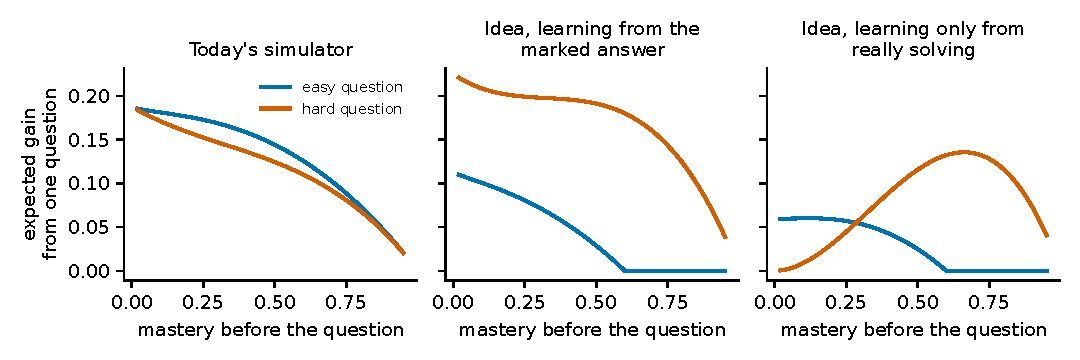
\includegraphics[width=\linewidth]{figs/f1_gain.pdf}
\caption{Expected mastery gain from one question, easy (blue) or hard (red), at each mastery level. Easy capped at 0.6; a failed hard question teaches nothing. Left: today's simulator, where easy always wins. Middle: Sir's idea, learning from the marked answer, where hard always wins. Right: Sir's idea, learning only from really solving, where easy wins at first and hard wins later.}\label{f:gain}
\end{figure}

\textbf{Trap 2: what a failed hard question teaches.} This one choice decides whether the switch exists (Figure~\ref{f:switch}). Looking at a single question, if a failed hard question teaches nothing, hard starts to give a bigger expected gain than easy at mastery \V{sw.0.4}, \V{sw.0.6} or \V{sw.0.8} for easy limits of 0.4, 0.6 and 0.8. With the 0.6 limit, if a failed hard question teaches about \V{sw.0.6.always} of the remaining gap or more (on my grid of 0.01 steps), hard is better from the very first question. This fits, but is not directly tested by, the studies in Section~7: hard material far beyond the learner teaches little, and trying problems before being taught gives a moderate benefit when the teaching follows.

\begin{figure}[H]\centering
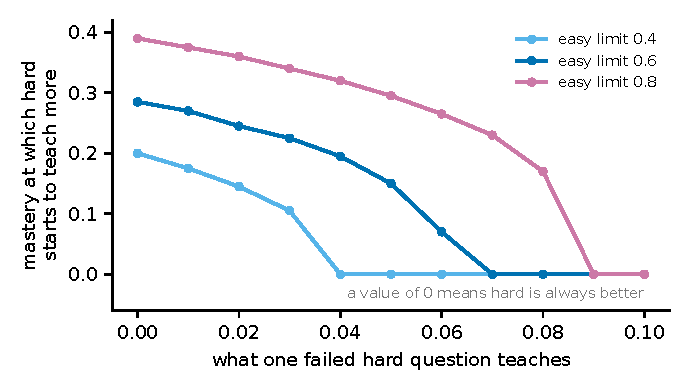
\includegraphics[width=0.62\linewidth]{figs/f2_switch.pdf}
\caption{For a single question: the mastery at which a hard question gives a bigger expected gain than an easy one, against what a failed hard question teaches. One line per easy limit. Zero means hard is better from the start.}\label{f:switch}
\end{figure}

\section{One concept: what is the best plan?}
Here every student is identical, starts at mastery 0.05, and the goal is mastery 0.9. Figure~\ref{f:switch} compared single questions. Here I ask a different question: which plan reaches 0.9 in the fewest questions overall? I computed the best possible plan exactly (a standard shortest-path calculation) and checked it with simulated students.

\textbf{The best plan is, in effect, a single switch: easy below a mastery level, hard above it.} The switch point is \V{s.cap.sw} in reading (b) and \V{s.slow.sw} in reading (a). It comes later than in Figure~\ref{f:switch} because the plan also counts what each question sets up for the next ones. With my setting, one solved hard question takes mastery from any level to at least 0.9 (it lands at $0.9 + 0.1m$). So on one concept the plan is really: raise mastery with easy questions until a hard question is likely enough to be solved, then wait for one solve. This best plan watches the student's true mastery, which a real tutor cannot see. So I also tried the best \emph{fixed} plan: ask $k$ easy questions, then only hard ones, with the best $k$. Figure~\ref{f:traj} shows the average student under each plan, and Table~\ref{t:sched} gives the counts.

\begin{figure}[H]\centering
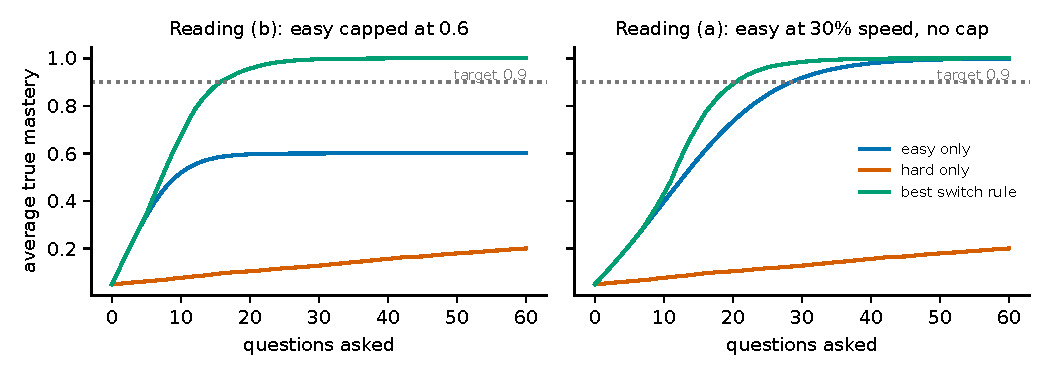
\includegraphics[width=\linewidth]{figs/f3_traj.pdf}
\caption{Average true mastery over the first 60 questions (4000 simulated students, failed hard questions teach nothing). Easy only stops at the cap in reading (b) and is slower in reading (a). Hard only barely moves, because a beginner almost never solves a hard question. Easy-then-hard is fastest in both. The average curve crosses 0.9 later than the average student does; Table~\ref{t:sched} gives the questions each student needs.}\label{f:traj}
\end{figure}

\begin{table}[H]\centering\small
\begin{tabular}{lcccc}
\toprule
 & \multicolumn{4}{c}{average questions to reach mastery 0.9}\\
Version & best switch & best fixed plan & easy only & hard only\\
\midrule
(b) easy capped at 0.6 & \V{s.cap.opt} & \V{s.cap.fix} (\V{s.cap.fixk} easy, then hard) & \V{s.cap.easy} & \V{s.cap.hardreach}\pc{} reach in 400\\
(a) easy at 30\pc{} speed & \V{s.slow.opt} & \V{s.slow.fix} (\V{s.slow.fixk} easy, then hard) & \V{s.slow.easy} & \V{s.slow.hardreach}\pc{} reach in 400\\
(b), failed hard teaches 0.05 & \V{s.capb.opt} & \V{s.capb.fix} (\V{s.capb.fixk} easy, then hard) & \V{s.capb.easy} & \V{s.capb.hard}\\
(a), failed hard teaches 0.05 & \V{s.slowb.opt} & \V{s.slowb.fix} (\V{s.slowb.fixk} easy, then hard) & \V{s.slowb.easy} & \V{s.slowb.hard}\\
\bottomrule
\end{tabular}
\caption{One concept. When a failed hard question teaches nothing (top two rows), the switch matters a lot. When it teaches 0.05 (bottom two rows), hard-only is about as good as the best plan, so there is little left to decide.}\label{t:sched}
\end{table}

\textbf{Different students need different switch points.} I then gave each student their own easy limit (0.4 to 0.8), hard-question jump, learning speed and starting mastery. Each student's best switch point ranged from \V{het.min} to \V{het.max} (median \V{het.med}; Figure~\ref{f:students}, left). The more the students' starting mastery varied, the more a tailored plan helped: the gap between the best tailored plan and the best single plan for everyone grew from \V{ad.0.3.gap} to \V{ad.0.85.gap} questions per concept (Figure~\ref{f:students}, right). I also tried a rule that sees only answers: ask hard; after a wrong hard answer, ask easy questions until one is answered right, then hard again. Against the best fixed plan it was \V{ad.0.3.phrase} and \V{ad.0.6.phrase} at the two narrower spreads, and \V{ad.0.85.phrase} at the widest. So it captured little of the gain. A tutor will need a proper estimate of mastery that accounts for difficulty. (This is a different rule from the ``easy until 3 right'' rule in Section~6.)

\begin{figure}[H]\centering
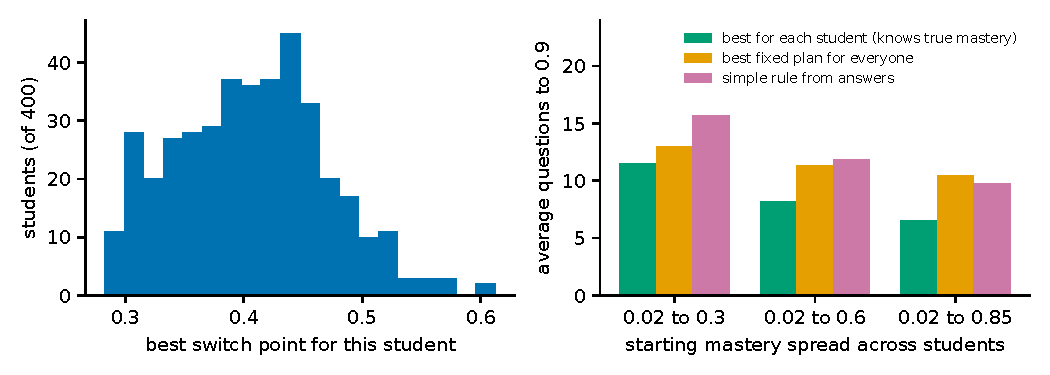
\includegraphics[width=\linewidth]{figs/f4_students.pdf}
\caption{Left: each student's best switch point (400 students). Right: average questions to mastery 0.9 for three plans, as students' starting mastery becomes more varied. Settings were chosen on 300 other students.}\label{f:students}
\end{figure}

\textbf{A warning about realism.} Under the best plan the simulated student answers correctly only about \V{succ.cap}\pc{} of the time. Theory puts the fastest learning near 85\pc{} correct (Wilson et al.). In a real practice system, learners rated the difficulty about right at roughly 60 to 70\pc{} correct, and learning was similar from 50\pc{} to 80\pc{} target success (Papou\v{s}ek et al.; Pel\'anek et al.). Our \V{succ.cap}\pc{} is below all of these. Our simulator has no penalty for frustration or quitting, so it can push students hard for free. Also, easy and hard questions differ little in accuracy in our answer model: at mastery 0.9 the chance of a right answer is \V{pr.0.9.e}\pc{} on an easy question and \V{pr.0.9.h}\pc{} on a hard one.

\section{The mastery test can be fooled by easy questions}
CurriculumTutor (Shabana et al., AIED 2022; ``the paper'' below) picks the next concept with a bandit, picks a random question inside it, and uses a running score to decide when a concept is learned. Each right answer adds about 1.3 points and each wrong answer takes away about 2, and the score never drops below zero. At about 7.8 points the concept is marked ``learned'' and is never asked again. From a score of zero this takes seven right answers in a row; after a wrong answer the leftover score counts, so fewer can be enough. Below, \emph{truly learned} means the student's hidden mastery is at least 0.8, and \emph{marked learned} means this test has fired.

The test treats every question in a concept as equally hard. With Sir's idea that is no longer true. I gave a student 200 easy questions only, with true mastery capped below 0.8, and ran the paper's test on the answers (1000 students per cap).

\begin{figure}[H]\centering
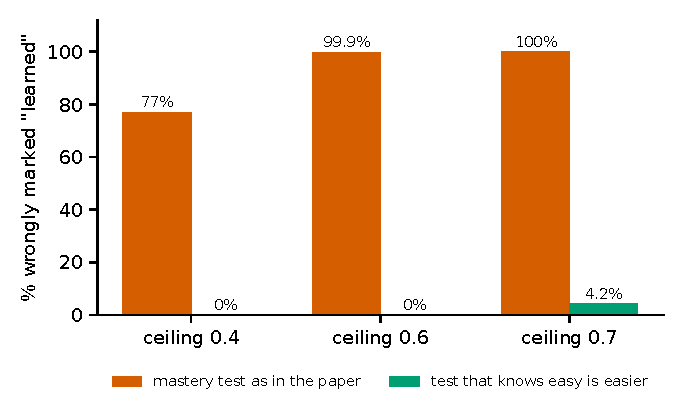
\includegraphics[width=0.62\linewidth]{figs/f5_cusum.pdf}
\caption{Share of students marked ``learned'' although their true mastery could never reach 0.8. Red: the paper's test as I implemented it (guess 0.25, slip 0.10). Green: the same test told that a student who has not learned the concept still gets 65\pc{} of easy questions right, not 25\pc{} (the idea behind KT-IDEM, Section~7; I chose 65\pc{} by hand).}\label{f:cusum}
\end{figure}

With caps of 0.4, 0.6 and 0.7, the paper's test wrongly marked the concept learned in \V{cu.0.4.b}\pc, \V{cu.0.6.b}\pc{} and \V{cu.0.7.b}\pc{} of runs (Figure~\ref{f:cusum}). Among those runs, the median was \V{cu.0.4.q}, \V{cu.0.6.q} and \V{cu.0.7.q} questions. The difficulty-aware version did so in \V{cu.0.4.a}\pc, \V{cu.0.6.a}\pc{} and \V{cu.0.7.a}\pc. This is a clean ``CurriculumTutor plus one change'' result, the kind of test Sir asked for.

\section{The 40-concept graph: can students reach the end?}
I used the shared 40-concept graph with the real simulated-student code and forgetting off, as the meeting notes asked. The deepest concept, G01, depends on 13 other concepts spread over six earlier levels (Figure~\ref{f:graph}). I call G01 and these 13 concepts \emph{G01's chain} (14 concepts; it branches, but every one is needed). ``Reaching the end'' means G01 and all 13 prerequisites are truly learned.

\begin{figure}[H]\centering
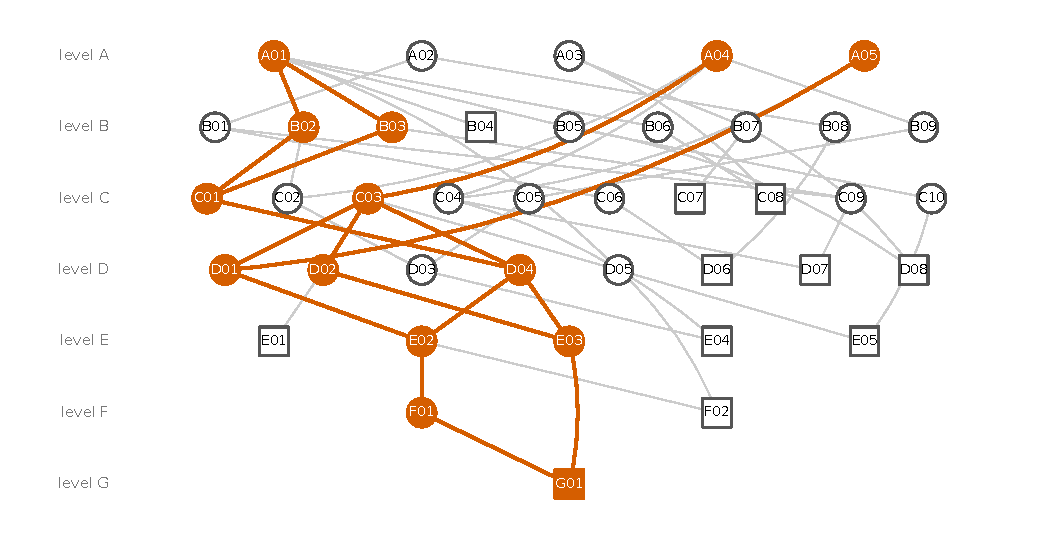
\includegraphics[width=0.92\linewidth]{figs/f6_graph.pdf}
\caption{The 40-concept graph. Filled: G01's chain. Squares: the 11 concepts that nothing depends on.}\label{f:graph}
\end{figure}

I compared three tutors. Two are \emph{best-case} tutors that can see the student's true mastery and move on when a concept reaches 0.8: one teaches only G01's chain, and one teaches the whole graph in order. The third is the real CurriculumTutor, which only sees answers.

\begin{figure}[H]\centering
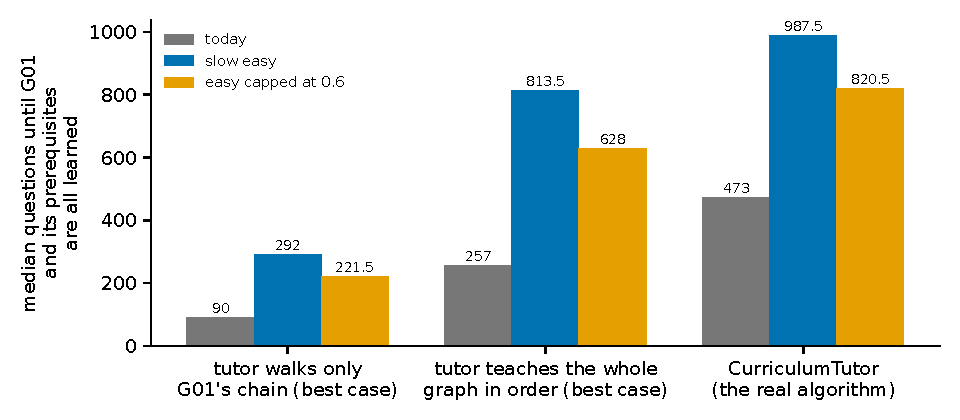
\includegraphics[width=0.85\linewidth]{figs/f7_reach.pdf}
\caption{Median questions until G01 and all its prerequisites are truly learned (200 students, question picked at random inside each concept, as in the paper). With Sir's idea, \V{f7.slow_bH0.ct.never}\pc{} (slow easy) and \V{f7.cap60_bH0.ct.never}\pc{} (capped easy) of CurriculumTutor's students had not got there after 2000 questions.}\label{f:reach}
\end{figure}

\textbf{What Figure~\ref{f:reach} shows.} With Sir's idea, every tutor needs many more questions than today; with slower learning settings that is expected. Teaching the whole graph instead of only G01's chain costs about \V{ratio.slow_bH0} times as much. CurriculumTutor needed \V{f7.slow_bH0.ct} (slow easy) and \V{f7.cap60_bH0.ct} (capped easy) questions, against \V{f7.current.ct} today. Within the usual 500 questions it got \V{f7.current.ct.r500}\pc{} of students to the end today, against \V{f7.slow_bH0.ct.n500} of 200 (slow easy) and \V{f7.cap60_bH0.ct.n500} of 200 (capped easy) with the idea. The students who never got there are stuck, not slow: every one of them (\V{stuck.slow_bH0.false} of \V{stuck.slow_bH0.n} with slow easy, \V{stuck.cap60_bH0.false} of \V{stuck.cap60_bH0.n} capped) had a concept wrongly marked learned, and the tutor had marked all 40 concepts learned and stopped asking. No extra student got there between question 1500 and 2000 (\V{stuck.slow_bH0.by1500} and \V{stuck.slow_bH0.by2000} of 200 with slow easy). A bigger budget will not help them; a more honest mastery test would.

\begin{figure}[H]\centering
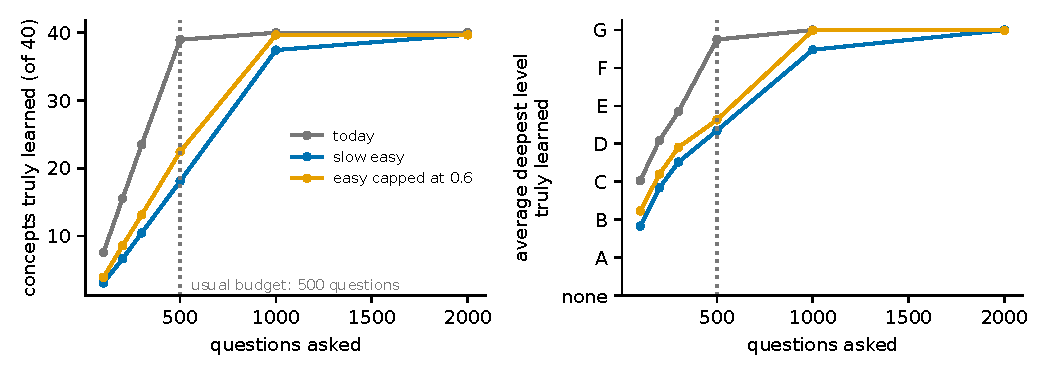
\includegraphics[width=\linewidth]{figs/f8_progress.pdf}
\caption{CurriculumTutor over time (100 students): concepts truly learned, and the average deepest level with a truly learned concept (the meeting's ``position in the graph''; this counts any concept at 0.8 or above, whether or not its prerequisites are learned). At the usual 500 questions, today's simulator has taught almost everything; with Sir's idea, students have learned about half the concepts.}\label{f:progress}
\end{figure}

At question 500 the average student had truly learned \V{f8.current.l500} concepts today, against \V{f8.slow_bH0.l500} (slow easy) and \V{f8.cap60_bH0.l500} (capped easy) with the idea (Figure~\ref{f:progress}).

\begin{table}[H]\centering\footnotesize
\begin{tabular}{>{\raggedright}p{3.4cm}ccccc}
\toprule
 & \multicolumn{4}{c}{best-case tutor teaching G01's chain; inside a concept it asks:} & whole graph\\
Version & easy only & hard only & random & easy, then & easy, then\\
 & & & & hard at 0.4 & hard at 0.4\\
\midrule
\TGraph
\bottomrule
\end{tabular}
\caption{Median questions until G01 is truly learned, best-case tutors (100 students). ``Easy, then hard at 0.4'' looks at true mastery, so it is a best case too. ``$>$2000 ($x$\pc)'' means only $x$\pc{} of students got there within 2000 questions. Figures~\ref{f:reach} and~\ref{f:bh} use 200 students, so the same setting can differ by a few questions.}\label{t:graph}
\end{table}

\textbf{When does a student reach the end quickly?} (Table~\ref{t:graph} and Figure~\ref{f:bh}.)
\begin{enumerate}[leftmargin=*]
\item \textbf{Every concept has both easy and hard questions.} If one difficulty cut-off is used for the whole graph, the early concepts get almost only easy questions and the deepest ones only hard questions. Then even the best-case chain tutor got only \V{abs.slow_bH0.switch}\pc{} (slow easy) or \V{abs.cap60_bH0.switch}\pc{} (capped easy) of students to G01 within 2000 questions.
\item \textbf{The tutor teaches only what the end needs.} Teaching only G01's chain is about \V{ratio.slow_bH0} times faster than teaching everything.
\item \textbf{Easy first, then hard.} When a failed hard question teaches nothing, hard only from a near-zero start gets almost nobody there. Easy only never finishes when easy is capped below 0.8.
\item \textbf{A failed hard question teaches at least a little} (Figure~\ref{f:bh}). At 0.02, hard only (\V{bh.02.hard} questions) already beats easy-then-hard (\V{bh.02.switch}).
\item \textbf{The student already knows something} (slow easy, best-case chain tutor). Starting at mastery 0.3, hard only takes \V{prior.0.3.hard} questions against \V{prior.0.3.switch} for easy-then-hard. Starting at 0.1, hard only takes \V{prior.0.1.hard}, and only \V{prior.0.1.hard.r}\pc{} get there within 2000.
\item \textbf{A faster learner.} \V{prof.fast}, \V{prof.avg} and \V{prof.slow} questions for fast, average and slow learners (slow easy, easy-then-hard).
\end{enumerate}
How strongly prerequisites slow learning hardly mattered (slow easy, easy-then-hard: \V{preq.min} to \V{preq.max} questions). That is only because these tutors wait until prerequisites are learned.

\begin{figure}[H]\centering
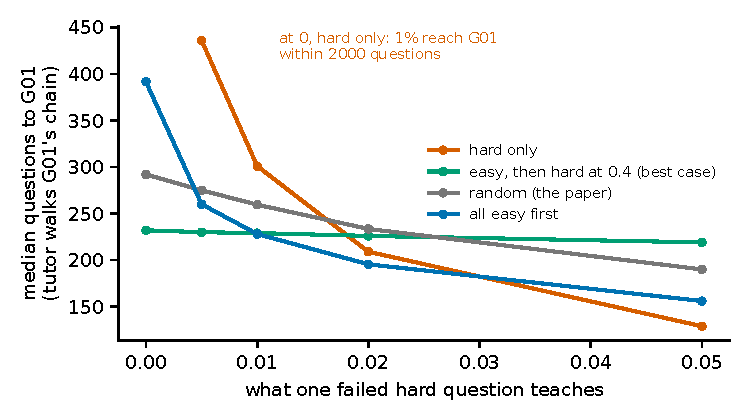
\includegraphics[width=0.68\linewidth]{figs/f9_bh.pdf}
\caption{What a failed hard question teaches, against median questions to G01 (slow easy, best-case tutor teaching G01's chain, 200 students). At zero, hard only gets only \V{bh.0.hardreach}\pc{} of students there within 2000 questions.}\label{f:bh}
\end{figure}

\textbf{Problems this exposed in our simulator}
\begin{itemize}[leftmargin=*]
\item \textbf{Prerequisites can be skipped.} Today a student whose weakest prerequisite is at 0 still learns at 20\pc{} of normal speed. A tutor that teaches G01 directly gets G01 to 0.8 in \V{dir.current} questions in today's simulator (\V{chain.current} through the chain), and in \V{dir.slow_bH0} with slow easy questions (\V{chain.slow_bH0} through the chain, easy-then-hard). If instead learning speed were simply multiplied by the weakest prerequisite, skipping would lose: \V{dir1.current} questions with only \V{dir1.current.r}\pc{} reaching, against \V{chain1.current} through the chain (today); \V{dir1.slow_bH0} with \V{dir1.slow_bH0.r}\pc{} reaching, against \V{chain1.slow_bH0} (slow easy). So ``reaching the end'' must include the prerequisites, or prerequisites must block learning.
\item \textbf{One solved hard question nearly masters a concept.} With my setting, a solved hard question closes 90\pc{} of the remaining gap. That is extreme. I reran the Section~6 comparisons with half that jump; their directions held.
\item \textbf{Students who start at exactly zero.} The simulator draws starting mastery around 0.05 and rounds negative values up to 0. A concept at exactly 0 can never be solved, so with hard only and nothing learned from failures it stays stuck forever. This affects only the hard-only results.
\end{itemize}

\section{All easy questions first, or random questions inside a concept?}
CurriculumTutor picks a random question inside a concept. I compared that with ``all easy first'': ask each of the concept's easy questions once, easiest first, then only hard ones. Each concept has 3 to 5 easy questions. The same 200 students were used for every plan, so each student can be compared with themselves. I did this first with the best-case tutor teaching G01's chain (Figure~\ref{f:ef}, Table~\ref{t:ef}, Figure~\ref{f:dose}), then inside CurriculumTutor itself (Figure~\ref{f:ct}).

\begin{figure}[H]\centering
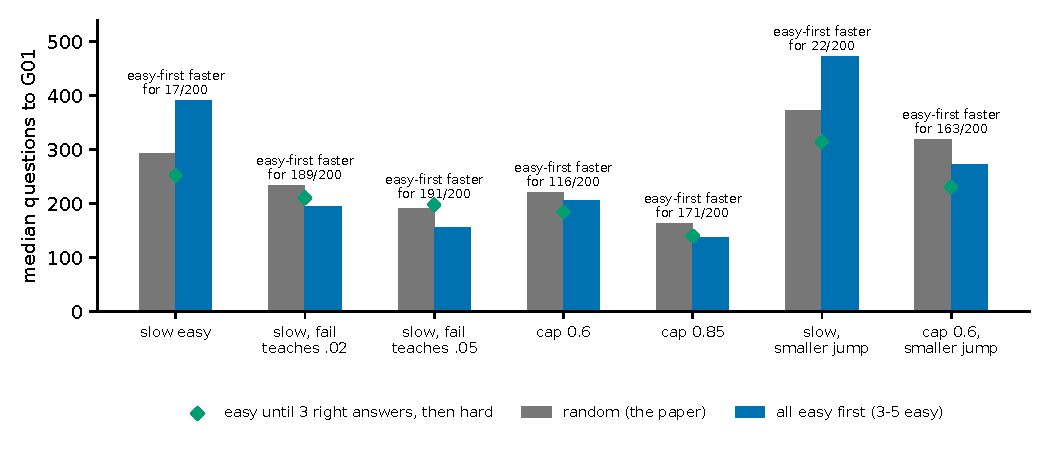
\includegraphics[width=\linewidth]{figs/f10_easyfirst.pdf}
\caption{Median questions to G01, best-case tutor teaching G01's chain. Grey: random (the paper). Blue: all easy first. Green diamond: easy until 3 right answers on that concept, then hard. The text shows for how many of the 200 students all-easy-first was faster than random.}\label{f:ef}
\end{figure}

\begin{table}[H]\centering\footnotesize
\setlength{\tabcolsep}{4pt}
\begin{tabular}{>{\raggedright}p{3.3cm}ccccccc}
\toprule
Version & random & all easy & easy first & paired & same easy Qs & easy until & best number\\
 & & first & faster/slower & difference & mixed in & 3 right & of easy first\\
\midrule
\TEasy
\bottomrule
\end{tabular}
\caption{Median questions to G01, best-case tutor teaching G01's chain, 200 students. ``Paired difference'' is the median over students of (all easy first minus random); negative means easy first is faster. ``Same easy Qs mixed in'' asks the same easy questions but mixed in with hard ones. The last column tries 2, 4, 8, 12 or 16 easy questions first (in brackets: its median). Numbers can differ slightly from Table~\ref{t:graph}, which uses 100 students.}\label{t:ef}
\end{table}

\textbf{Mostly it is how many easy questions are asked; asking them first also helps.}
\begin{itemize}[leftmargin=*]
\item Today's simulator: no difference (\V{ef.cur.rnd} against \V{ef.cur.ef} questions).
\item \textbf{When easy questions are slow and a failed hard question teaches nothing, all-easy-first loses} (\V{ef.slow_bH0.ef} against \V{ef.slow_bH0.rnd}; slower for \V{ef.slow_bH0.l} of 200 students). Three to five slow easy questions leave the student at mastery of only about \V{hand.slow_bH0} when the hard questions start. The student then waits for a rare real solve of a hard question while learning nothing. Random keeps mixing in easy questions, which keep teaching.
\item \textbf{When a failed hard question teaches a little, or easy questions are capped, all-easy-first wins} (only narrowly with the 0.6 cap and the full hard jump). Random keeps asking easy questions after they have stopped helping (capped easy), or after hard questions have started to help more (slow easy).
\item \textbf{Asking the easy questions first beats mixing the same ones in.} In \V{efmix.clear} of \V{nvers} versions, many more students were faster with easy first than with mixing (at least \V{efmix.minw} against at most \V{efmix.maxl}; the rest tied). In the remaining one (\V{efmix.close.ver}) the two were tied: \V{efmix.close.w} students were faster with easy first and \V{efmix.close.l} with mixing (medians \V{efmix.close.ef} and \V{efmix.close.mix}).
\item \textbf{The right number of easy questions depends on the version} (Figure~\ref{f:dose}). When a failed hard question teaches nothing: about \V{ef.slow_bH0.bestk} with slow easy (\V{ef.slow_bH0.k8} questions with 8 was almost as good), and about \V{ef.cap60_bH0.bestk} with capped easy. When a failed hard question teaches 0.05: \V{ef.slow_bH05.bestk} or fewer, and hard only (\V{bh.05.hard} questions) was fastest. When a concept has fewer easy questions than the number asked, its 3 to 5 easy questions are repeated in turn.
\item \textbf{A practical rule works well.} ``Easy until 3 right answers on that concept, then hard'' beat random in \V{e3.wins} of \V{nvers} versions. It lost only when a failed hard question teaches 0.05, where easy questions are not needed at all.
\end{itemize}

\begin{figure}[H]\centering
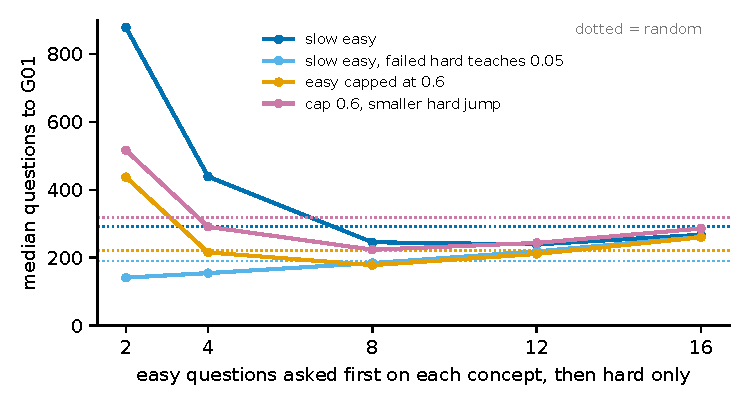
\includegraphics[width=0.74\linewidth]{figs/f11_dose.pdf}
\caption{Median questions to G01 when a fixed number of easy questions is asked first on each concept, then only hard ones (easy questions repeated in turn if needed). Dotted lines show random for the same version.}\label{f:dose}
\end{figure}

\textbf{Inside CurriculumTutor, the bigger effect is on the mastery test} (Figure~\ref{f:ct}). The test counts right answers and ignores difficulty, and a concept marked ``learned'' is never asked again.
\begin{itemize}[leftmargin=*]
\item \textbf{Random fooled the test more in every version} (\V{fd.rnd.gt} of \V{nvers}). By question 2000, random had wrongly marked \V{fd.rnd.min7} to \V{fd.rnd.max7} concepts per student as learned, against \V{fd.ef.min} to \V{fd.ef.max} for all-easy-first. Asking 16 easy questions first was worst (\V{fd.k16.min} to \V{fd.k16.max}). The test is fooled much more when many easy questions are asked after the student is partly there.
\item \textbf{The cost is real.} With easy capped at 0.6 and the smaller hard jump, only \V{clo.rnd.capb1}\pc{} of students under random ever truly learned all of G01's chain, against \V{clo.ef.capb1}\pc{} with all-easy-first and \V{clo.e3.capb1}\pc{} with ``easy until 3 right''.
\item \textbf{A test that only counts answers to hard questions removes most of the problem} (at most \V{cth.rnd.max} wrong verdicts per student for random). With slow easy, it raised the share of random's students who reach the end from \V{ct.rnd.slow.reach}\pc{} to \V{cth.rnd.slow.reach}\pc, but the median rose from \V{ct.rnd.slow} to \V{cth.rnd.slow} questions. Combined with ``easy until 3 right'', the median was \V{cth.e3.slow}.
\item \textbf{On the whole chain under CurriculumTutor,} all-easy-first was slower than random with slow easy (faster for \V{ctp.slow_bH0.w}, slower for \V{ctp.slow_bH0.l} of 200) and faster with capped easy (\V{ctp.cap60_bH0.w} against \V{ctp.cap60_bH0.l}). ``Easy until 3 right'' beat random in both (\V{cte3.slow_bH0.w} against \V{cte3.slow_bH0.l}, and \V{cte3.cap60_bH0.w} against \V{cte3.cap60_bH0.l}), and in \V{cte3.wins7} of \V{nvers} versions overall; it lost only when a failed hard question teaches 0.05.
\end{itemize}

\begin{figure}[H]\centering
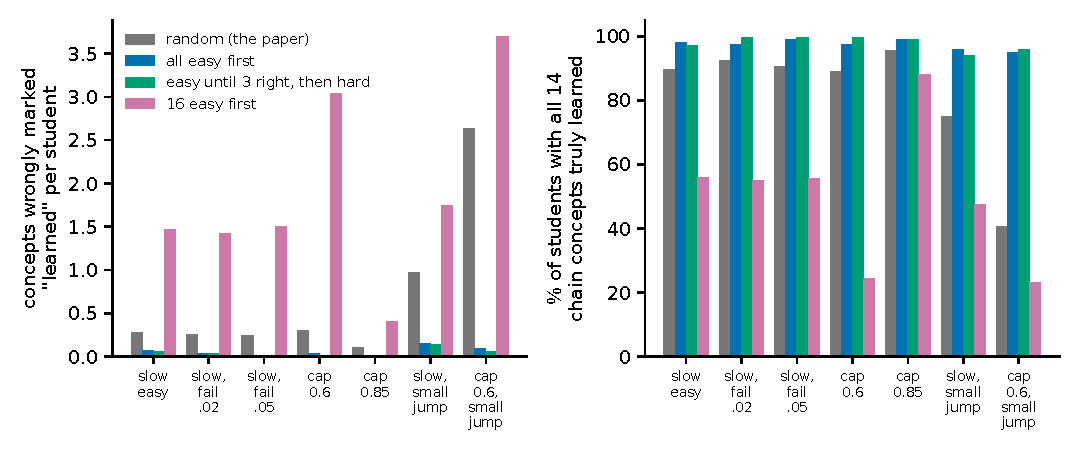
\includegraphics[width=\linewidth]{figs/f12_ct.pdf}
\caption{CurriculumTutor, 200 students, after 2000 questions, all seven versions. Left: concepts wrongly marked ``learned'' per student. Right: share of students whose 14 chain concepts are all truly learned.}\label{f:ct}
\end{figure}

\textbf{What this means for my part (difficulty inside a concept).} Because easy and hard questions now teach differently, the paper's random choice inside a concept is no longer neutral. Replacing it with ``easy until 3 right answers, then hard'' is the kind of ``CurriculumTutor plus one change'' Sir asked for: inside CurriculumTutor it was faster than random in \V{cte3.wins7} of \V{nvers} versions, and it made the mastery test far more honest. How many easy questions to ask is still open, and it depends on Sir's answer about failed hard questions.

\section{What other studies found}
The meeting notes asked me to record what data and measures each paper used. Every entry below was checked against the paper's own text, except Sinha \& Kapur 2021 (abstract only) and Papou\v{s}ek et al.\ 2016 (checked against the authors' extended report).

{\small
\setlength{\tabcolsep}{4pt}
\begin{longtable}{>{\raggedright}p{2.7cm}>{\raggedright}p{3.1cm}>{\raggedright}p{5.4cm}>{\raggedright\arraybackslash}p{4.3cm}}
\toprule
Paper & Data and measure & What they found & What it means for us\\
\midrule\endhead
Wilson et al.\ 2019, Nature Communications & Theory and computer learners; no human test. Learning speed against training error & Learning is fastest at about 85\pc{} correct. Very easy items give almost no learning signal; at a fixed difficulty, progress becomes extremely slow. & Supports ``easy is slow'' (reading (a)) more than a hard cap.\\
Metcalfe \& Kornell 2003, JEP: General & Adults studying word pairs in the lab. Recall gained per second of study & Easy items level off after about one second; medium items keep gaining longer. More than ten times the study time on difficult items gave no gain. & Easy items are learned fast and then stop paying; items far beyond the learner give almost nothing. (These are different words, not easy and hard questions on one concept.)\\
Kornell \& Metcalfe 2006, JEP: LMC & Spanish--English pairs people had just failed; restudied with the answer shown. Final recall & Restudying the easiest unlearned items beat restudying the hardest (.28 vs .12, and .25 vs .15). & Material far beyond the student teaches little, even with the answer shown.\\
Pashler \& Mozer 2013, JEP: LMC & Seven category-learning experiments. Final test accuracy & Easy-to-hard training helped a lot only when the task had distracting features (69.0\pc{} vs 49.0\pc{} for hard only); otherwise no reliable difference (67.8\pc{} vs 66.1\pc). & Readiness matters in some tasks, not all.\\
Sinha \& Kapur 2021, Review of Educational Research & Meta-analysis, 53 studies (abstract only) & Trying problems before being taught beat teaching first, a moderate effect (effect size $g = 0.36$); reversed for grades 2--5. & A failed attempt can help when teaching follows it.\\
Papou\v{s}ek et al.\ 2016, ITS & Geography practice website, about 37,000 learners, four randomised target success rates (95, 80, 65, 50\pc). Learning curves, dropout & The easiest level (target 95\pc{} correct) learned least, though the authors say dropout may explain part of this; the harder levels were similar. Easier kept more learners in the short run. Learners rated the difficulty about right at roughly 70\pc{} correct. & Too easy is bad, but harder is not always better.\\
Pel\'anek et al.\ 2017, UMUAI & Same website and experiment. Model fit and learning & In their tracing rule a right answer on a hard item raises the knowledge estimate more. Harder practice was better, mainly against the easiest arm. & Supports a difficulty-aware mastery test; only indirectly Sir's learning rule.\\
Lomas et al.\ 2013, CHI & Number-line game, about 10,000 sessions and 70,000 players. Play time, learning rate & Easier targets meant more play (34\pc{} more estimates) but slower learning. & Real students quit when it is too hard; our simulator has no quitting.\\
de Lima et al.\ 2020, Spanish J.\ of Psychology & Swahili--Portuguese word pairs, test after 48 hours & Practice testing helped easy items more in one experiment (.26 vs .19, $p = .05$); the second leaned the other way (.28 vs .18, not significant). & No clear bonus for hard items; test several sizes.\\
Agarwal 2019, J.\ of Educational Psychology & College and 6th-grade classes; fact vs higher-order quizzes. Delayed tests & Fact quizzes did not help the higher-order test (46\pc{} vs 44\pc); higher-order quizzes did (72\pc). But higher-order quizzes did not help the fact test (53\pc{} vs 78\pc{} for fact quizzes), and mixed quizzes were best in 6th grade. & Supports a cap, but hard practice did not replace easy practice either: closer to two separate parts of mastery than one number with a cap.\\
Pardos \& Heffernan 2011 (KT-IDEM), UMAP & ASSISTments and Cognitive Tutor data. AUC (how well right answers are predicted) & Giving each question its own guess and slip beat plain Bayesian Knowledge Tracing (BKT) on 9 of 10 ASSISTments sets (average AUC 0.669 to 0.699). No overall gain on Cognitive Tutor data (0.646 vs 0.644); gains only where questions had enough answers. & A tracer that knows difficulty: a likely fix for the fooled mastery test, but per-question settings need enough data.\\
Doroudi \& Brunskill 2019, LAK & Simulated BKT and gradual learners. True mastery when declared & BKT declared mastery when the true chance of a right answer was only 0.45 to 0.60. & The same symptom (mastery declared too early) from a related cause: the tracer assumes the wrong learning model.\\
Koedinger et al.\ 2023, PNAS & 27 datasets, about 1.3 million answers, 6,946 learners & Students differ a lot in what they know at the start, and very little in learning rate. & When we add randomness, vary starting knowledge first.\\
Clement et al.\ 2015 (ZPDES), JEDM & 1,000 simulated students; about 400 children aged 7--8 & Simulated students had their own maximum level per skill; adapting helped most when students differed. & A precedent for a per-student cap.\\
Doroudi et al.\ 2017, Learning @ Scale & Fractions tutor. Simulated vs real post-test & One simulator predicted a huge gain; the real classroom showed none. & Test our tutors on several simulator versions, not one.\\
\bottomrule
\end{longtable}}

No study I found tests Sir's exact design with real learners. The closest precedents are simulators. In the 2013 preprint of Clement et al., practice moves a simulated student's level toward the exercise's level, which caps easy practice (reading (b)); I could not confirm this in their code. In Segal et al.\ (AIED 2018), the gain from a right answer grows with the question's difficulty, which makes easy practice slow (reading (a)). Most evidence supports a slow, levelling-off gain from easy questions rather than a hard cap, so the cap should be presented as our own assumption.

\section{What I propose next (not started)}
\begin{enumerate}[leftmargin=*]
\item Agree the decisions in Section~9 with Sir.
\item Add the easy/hard rule to the shared simulator as new options. Their default values must reproduce today's results exactly, with a test, so Sanved's results do not move.
\item Rerun, in the shared simulator and with Sir's chosen settings, the three experiments in this note: does difficulty matter at all; the mastery test, with plain BKT as the baseline and a difficulty-aware version (BKT with a guess and slip per question, as in KT-IDEM, or counting only hard answers) as the one change; and CurriculumTutor with ``easy until 3 right answers, then hard'' against the paper's random choice.
\item Then add randomness between students, starting with prior knowledge.
\end{enumerate}
Steps 1 to 3 are tight for the 31 October report; if time runs short, the mastery test and the easy-first comparison come first. Step 4 can go on the poster.

\section{Questions for Sir}
The first three matter most.
\begin{enumerate}[leftmargin=*]
\item \textbf{What should a failed hard question teach:} nothing, a little (2\pc{} of the remaining gap), or more (5\pc, for example if the tutor shows a worked solution after a wrong answer)? This one choice decides most results (Figures~\ref{f:switch} and~\ref{f:bh}).
\item \textbf{Slow or capped?} Should easy questions reach full mastery slowly, or only up to a limit? If a limit, what value? A limit at or below 0.8 means easy questions alone can never finish a concept.
\item \textbf{Learning from luck:} should a student learn only from really solving a question, and not from a lucky right guess? (If not, hard questions win at every level; Figure~\ref{f:gain}.)
\item \textbf{Labels:} should every concept have its own easy and hard questions, or should one difficulty cut-off be used for the whole graph? (With one cut-off, even the best-case tutor got only \V{abs.slow_bH0.switch}\pc{} (slow easy) or \V{abs.cap60_bH0.switch}\pc{} (capped easy) of students to G01 within 2000 questions.) Two levels, or Easy, Medium and Hard as in the last meeting's notes?
\item \textbf{Prerequisites:} should weak prerequisites block learning, or only slow it? And does ``reaching the end'' mean the end concept alone, or the end concept with all its prerequisites?
\item \textbf{Mastery test:} should a concept count as learned only after right answers on hard questions, or should the test be told how easy each question is (BKT with a guess and slip per question, as in KT-IDEM)? Counting only hard answers removed most wrong verdicts, but made the paper's random choice slower.
\item \textbf{How many easy questions before hard:} a fixed number, until some right answers, or from the tutor's estimate of mastery?
\item \textbf{Realism:} is a 90\pc{} jump from one solved hard question too big? Should the simulator include quitting, given that students are right only about \V{succ.cap}\pc{} of the time under the best plan?
\item \textbf{Budget:} with the idea, CurriculumTutor needed \V{f7.slow_bH0.ct} and \V{f7.cap60_bH0.ct} questions (median), against \V{f7.current.ct} today. Keep 500, or raise it?
\item \textbf{Randomness:} should students differ from each other (their own settings, starting knowledge first), or should each answer's learning be noisy, or both?
\end{enumerate}

\section{How I checked the numbers, and the limits}
\textbf{Checks.} Every simulation result in this note is produced by scripts from saved result files; the model settings and the literature numbers are written by hand. Separate automated re-runs audited the code against the real simulator and rebuilt the main simulations independently; their results matched within random noise. Further automated passes recomputed every headline number from the raw results and checked the literature table against the papers. Two mistakes were caught and fixed: CurriculumTutor was first measured on G01 alone instead of G01 with its prerequisites, and one extra test used different easy/hard labels for the tutor and the student.

\textbf{Limits.} All settings are my guesses. The best-case tutors see true mastery when deciding to move on, so they are optimistic; the fixed 0.4 switch is not always optimal, and simple answer-based rules sometimes beat it. Forgetting is off. There is one graph, no quitting or frustration, and a low success rate. A solved hard question is very powerful with my setting, though the Section~6 directions held with half the jump.

\textbf{AI use.} These notes, the simulations and the checks were prepared with help from an AI assistant (Claude).

\appendix
\section{Settings used}
{\small\begin{tabularx}{\linewidth}{>{\raggedright}p{3.6cm}>{\raggedright\arraybackslash}X}
\toprule
Chance of really solving & $m^{1+1.2d}$; easy $d = 0.2$ and hard $d = 0.8$ on one concept; the graph's own difficulties on the graph\\
Observed answer & right with chance 0.93 if solved, 0.25 (a guess) if not\\
Easy question & gain $0.45$ (solved) or $0.10$ (not) $\times$ speed $\times$ (limit $-$ mastery)\\
Reading (a) & speed 0.3, limit 1\\
Reading (b) & speed 1, limit 0.6 (also 0.85)\\
Hard question & solved: gain $0.9\times(1-m)$ (``smaller jump'': $0.45\times(1-m)$); failed: what it teaches $\times(1-m)$, 0 by default\\
Prerequisites & gain $\times$ (0.2 + 0.8 $\times$ weakest prerequisite), as in today's simulator\\
Learned & true mastery $\geq 0.8$ on the graph; target 0.9 in the one-concept study\\
Easy/hard on the graph & questions at or below the concept's median difficulty are easy (3 to 5 per concept)\\
Students & 100 or 200 per setting on the graph, the same students across plans; forgetting off\\
\bottomrule
\end{tabularx}}

\section{Files}
Everything is in \texttt{experiments/difficulty/} on the branch \texttt{difficulty}, made from \texttt{main}. The folder \texttt{simcore/} holds an unchanged copy of the simulator files the study needs (from Sanved's reorganised simulator on the \texttt{forgetting} branch, commit \texttt{d95830c}; see \texttt{simcore/PROVENANCE.md}), so the study does not depend on that branch. \texttt{make\_single.py}, \texttt{make\_single2.py}, \texttt{run\_grid.py}, \texttt{run\_ef.py} and \texttt{make\_extra.py} write the result files into \texttt{data/}. \texttt{make\_figs.py} and \texttt{make\_numbers.py} turn those files into every figure, table and simulation number in this note. \texttt{run\_all.sh} runs all of it (about 5 minutes). The scripts only import that copy; they do not change it, and nothing outside the folder changes.

\end{document}
